\chapter{If-Conversion \Author{C. Bruel}}
\label{chapter:if_conversion}
\inputpath{part4}{if_conversion}
\inputprogress

\newcommand{\annotation}[1]{%
  \marginpar{\small\itshape\color{red}#1}}

%\setcounter{tocdepth}{3} 
%\tableofcontents

% remember
% Check entry vs head in the examples
% example 21.9(b) x=psi (T ? x1, p bar ? x2)
% example 21.9(c) x=psi (T ? x1, p bar ? x2)

%\section{Introduction}

 Very Large Instruction Word (VLIW)\index{Very Long Instruction Word, VLIW} or Explicitly Parallel Instruction Computing (EPIC) architectures make Instruction Level Parallelism (ILP)\index{Instruction Level Parallelism, ILP} visible within the Instruction Set Architecture (ISA), relying on static schedulers\index{scheduling} to organize the compiler output such that multiple instructions can be issued in each cycle.

If-conversion\index{if-conversion} is the process of transforming a control-flow region with conditional branches, into an equivalent predicated\index{predicated execution} or speculated\index{speculative execution} sequence of instructions (into a region of Basic Blocks, possibly single) referred to as a Hyperblock. 
If-converted code replaces control dependencies\index{dependence, control-} by data dependencies\index{dependence, data-}, and thus exposes Instruction Level Parallelism\index{parallelism} very naturally within the new region at the software level.

Removing control hazards improves performance in several ways: 
Removing the misprediction penalty, the instruction fetch throughput is increased and the instruction cache locality improved. 
Enlarging the size of basic blocks allows earlier execution of long latency operations and the merging of multiple control-flow paths into a single flow of execution, that can later be exploited by scheduling frameworks such as VLIW scheduling, hyperblock scheduling or modulo scheduling.\index{scheduling}

Consider the simple example given in Figure~\ref{fig:example1}, that represents the execution of an \texttt{if-then-else-end} statement on a 4-issue processor with non-biased branches. 
In this figure, $r=q\cond r_1:r_2$ stands for a \texttt{select}\index{select, instruction} instruction where $r$ is assigned $r_1$ if $q$ is true, and $r_2$ otherwise. 
With standard basic block ordering, assuming that all instructions have a one cycle latency, the schedule height goes from five cycles in the most optimistic case, to six cycles. 
After if-conversion the execution path is reduced to four cycles with no branches, regardless of the test outcome, and assuming a very optimistic one cycle branch penalty. 
The main benefit here is that it can be executed without branch disruption.

\begin{figure}
  \subfloat[Control flow] {
    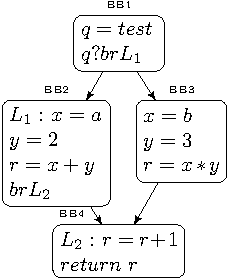
\includegraphics[scale=0.9]{specul}
    \label{fig:orig}
  }
  \subfloat[with basic block ordering] {
    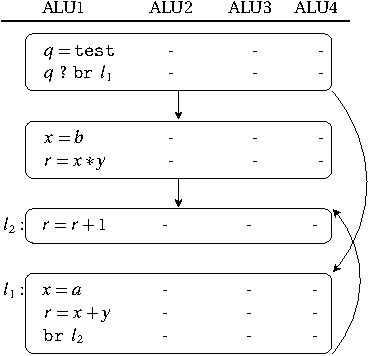
\includegraphics[scale=0.9]{specul-linear}
  }

  \subfloat[After if-conversion] {
    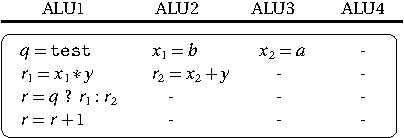
\includegraphics[scale=0.9]{specul-ifconverted}
  }
\caption{Static schedule of a simple region on a 4-issue processor. }
\label{fig:example1}
\end{figure}

From this introductory example, we can observe that:
\begin{itemize}
\item the two possible execution paths have been merged into a single execution path, implying a  better exploitation of the available resources;  
\item the schedule height has been reduced, because instructions can be control speculated before the branch;\index{speculation}
\item the variables have been renamed, and a \textit{merge} pseudo-instruction has been introduced.
\end{itemize}

Thanks to SSA, the merging point is already materialized in the original control flow as a $\phi$ pseudo-instruction, and register renaming was performed by SSA construction. 
Given this, the transformation to generate if-converted code seems natural locally. 
Exploiting those properties on larger scale control-flow regions requires a framework that we will develop further.

\subsection{Architectural requirements}

The \textit{merge} pseudo operations need to be mapped to a conditional form of execution in the target's architecture. As illustrated in Figure~\ref{fig:pred} we differentiate the three following models of conditional execution:
\begin{itemize}
\item \emph{Fully predicated execution}: Any instruction can be executed conditionally on the value of a predicate operand.\index{predication, full}
\item \emph{(Control) speculative execution}: The instruction is executed unconditionally, and then committed using conditional moves (\texttt{cmov} or \texttt{select}) instructions.\index{speculation}
\item \emph{Partially predicated execution}: Only a subset of the ISA is predicated, usually memory operations that are not easily speculated; other instructions are speculated.
\end{itemize}\index{predication, partial}
In this figure, we use the notation $r = c \cond r_1:r_2$, to represent a \texttt{select}\index{select, instruction} like operation. 
Its semantic is identical to the gated\index{gated instruction} $\phiif$-function\index{$\phiif$-function} presented in Chapter~\ref{chapter:vsdg}: 
$r$ takes the value of $r_1$ if $c$ is true, $r_2$ otherwise. 
Similarly, we also use the notation $c \cond r = op$ to represent the predicated execution of $op$ if the predicate $c$ is true; 
$\overline{c} \cond r = op$ if the predicate $c$ is false.

\begin{figure}[h]
\footnotesize
\subfloat[fully predicated]{
\begin{tabular}[t]{p{0.20\textwidth}}
$p \cond x = a + b $ \\
$\overline{p} \cond x = a * b $\\
~ 
\end{tabular}
}
\hfill
\subfloat[speculative using \emph{select}]{
\begin{tabular}[t]{p{0.27\textwidth}}
$t_1 = a + b $ \\
$t_2 = a * b $ \\
$x= p \cond t_1 : t_2 $ 
\end{tabular}
} \hfill
\subfloat[speculative using \emph{cmov}]{
\begin{tabular}[t]{p{0.27\textwidth}}
$x = a + b $ \\
$t = a * b $ \\
$x = \texttt{cmov}\ p,t$ 
\end{tabular}
}
\caption{Conditional execution using different models}
\label{fig:pred}
\end{figure}

To be speculated, an instruction must not have any side effects, or hazards. 
For instance, a memory load must not trap because of an invalid address. 
Memory operations are a major impediment to if-conversion. 
This is regrettable, because as any other long latency instructions, speculative loads can be very effective to fetching data earlier in the instruction stream, reducing stalls. 
Modern architectures provide architectural support to dismiss invalid address exceptions. 
Examples are the \texttt{ldw.d} dismissible load operation in the Multiflow Trace series of computers, or in the STMicroelectronics ST231 processor, but also the speculative load of the Intel IA64. 
The main difference is that with a dismissible model, invalid memory access exceptions are not delivered, which can be problematic in an embedded or kernel environment that relies on memory exception for correct behavior. 
A speculative model allows to catch the exception thanks to the token bit check instruction. 
Some architectures, such as the IA64, offer both speculative and predicated memory operations.\index{dismissible model} Stores can also be executed conditionally by speculating part of their address value, with additional constraints on the ordering of the memory operations due to possible alias between the two paths. 
Figure~\ref{fig:spec} shows examples of various forms of speculative memory operations.

Note that the \texttt{select} instruction is an architecture instruction that does not need to be replaced during the SSA destruction phase. 
If the target architecture does not provide such gated instruction\index{gated instruction}, it can be emulated using two conditional moves\index{conditional move}. 
This translation can be done afterwards, and the \texttt{select} instruction still be used as an intermediate form. 
It allows the program to stay in full SSA form where all the data dependencies are made explicit, and can thus be fed to all SSA optimizers.

\begin{figure}[h]
\subfloat[IA64 speculative load]{\index{load, speculative}
\begin{minipage}[b]{0.30\textwidth}
$t = \texttt{ld.s(\textit{addr})} $ \\
$\texttt{chk.s (t)} $\\
$p \cond x = t$ 
\end{minipage}
}\hfill
\subfloat[Multiflow/ST231 dismissible load]{\index{load, dismissible}
\begin{minipage}[b]{0.32\textwidth}
$t = \texttt{ldw.d(\textit{addr})} $ \\
$x = \texttt{select}\:p \cond t : x $ \\
~
\end{minipage}
    }\\
\subfloat[base store hoisting]{
\begin{minipage}[b]{0.33\textwidth}
$x=\texttt{select}\:p \cond \textit{addr} : \textit{dummy} $ \\
$\texttt{stw} (x, \textit{value}) $ 
\end{minipage}
}\hfill
\subfloat[index store hoisting]{
\begin{minipage}[b]{0.32\textwidth}
$\textit{index}=\texttt{select}\:p \cond i : j $ \\
$\texttt{stw} (x[\textit{index}], \textit{value}) $ 
\end{minipage}
}
\caption{Examples of speculated memory operations}
\label{fig:spec}
\end{figure}




This chapter is organized as follows: 
we begin by describing the SSA techniques to transform a CFG region in SSA form to produce an if-converted SSA representation using speculation. 
We then describe how this framework is extended to use predicated instructions, using the $\psi$-SSA form presented in Chapter~\ref{chapter:psi_ssa}. 
Finally, we outline a global framework to pull together those techniques, incrementally enlarging the scope of the if-converted region to its maximum beneficial size.

\section{Basic transformations}
\label{sec:basic}

Unlike global approaches, that identify a control-flow region and if-convert it in one shot, the technique described in this chapter is based on incremental reductions. 
To this end, we consider basic SSA transformations whose goal are to isolate a simple diamond-DAG structure (informally an \texttt{if-then-else-end}) that can be easily if-converted. 
The complete framework, that identifies and incrementally performs the transformation, is described in Section~\ref{sec:if_conversion:hyperblock}.

\subsection{SSA operations on basic blocks}

The basic transformation that actually if-converts the code is the \emph{$\phi$~removal}\index{$\phi$ removal, reduction} that takes a simple diamond-DAG as an input, i.e., a single-entry-node/single-exit-node (SESE)\index{single-entry-node/single-exit-node, SESE} DAG with only two distinct forward paths from its entry node to its exit node. 
The $\phi$~removal consists in (1) speculating the code of both branches in the entry basic block (denoted \textit{head}); 
(2) then replacing the \phifun by a \texttt{select}; 
(3) finally, simplifying the control flow to a single basic block. 
This transformation is illustrated in Figure~\ref{fig:phi_rem}.
\begin{figure}[h]
  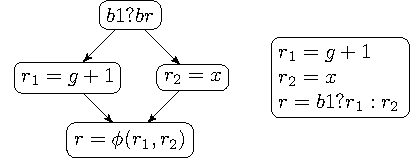
\includegraphics[scale=0.9]{phi_removal}
  \caption{$\phi$~removal\label{fig:phi_rem}}
\end{figure}

The goal of the \emph{$\phi$ reduction}\index{$\phi$ reduction, reduction} transformation is to isolate a diamond-DAG from a structure that resembles a diamond-DAG but has side entries to its exit block. 
This diamond-DAG can then be reduced using the $\phi$~removal transformation. 
Nested \texttt{if-then-else-end} in the original code can create such a control flow region. 
One can notice the similarity with the nested arity-two $\phiif$-functions\index{$\phiif$-function} used for gated-SSA\index{Gated-SSA form} (see Chapter~\ref{chapter:vsdg}). 
In the most general case, the joint node of the considered region has $n$ predecessors with \phifuns of the form $B_0:r=\phi(B_1:r_1,B_2:r_2,\dots,B_n:r_n)$, and is such that removing edges from $B_3,\dots, B_n$ would give a diamond-DAG. 
After the transformation, $B_1$ and $B_2$ point to a freshly created basic block, say $B_{12}$, that itself points to $B_0$; 
a new variable $B_{12}:r_{12}=\phi(B_1:r_1,B_2:r_2)$ is created in this new basic block; 
the \phifun in $B_0$ is replaced by $B_0:r=\phi(B_{12}:r_{12},\dots,B_n:r_n)$. 
This is illustrated in Figure~\ref{fig:phi_red}.
\begin{figure}[h]
  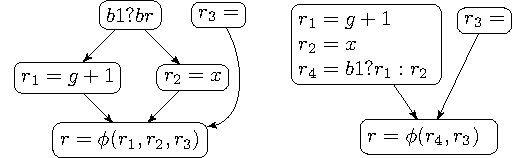
\includegraphics[scale=0.9]{phi_reduction}
  \caption{\label{fig:phi_red}$\phi$ reduction}
\end{figure}

The objective of \emph{path duplication}\index{path duplication} is to get rid of all side entry edges that avoid a single-exit-node region to be a diamond-DAG. 
Through path duplication, all edges that point to a node different than the exit node or to the willing entry node, are ``redirected'' to the exit node. 
$\phi$~reduction can then be applied to the obtained region. 
More formally, consider two distinguished nodes, named \textit{head} and the single exit node of the region \textit{exit}, such that there are exactly two different control-flow paths from \textit{head} to \textit{exit}; 
consider (if exists), the first node $\textit{side}_i$ on one of the forward path $\textit{head}\rightarrow \textit{side}_0\rightarrow\dots\textit{side}_p\rightarrow\textit{exit}$ that has at least two predecessors. 
The transformation duplicates the path $P=\textit{side}_i\rightarrow\dots\rightarrow\textit{side}_p\rightarrow\textit{exit}$ into $P'=\textit{side'}_i\rightarrow\dots\rightarrow\textit{side'}_p\rightarrow\textit{exit}$ and redirects $\textit{side}_{i-1}$ (or $\textit{head}$ if $i=0$) to $\textit{side'}_i$. 
All the \phifuns that are along $P$ and $P'$ for which the number of predecessors have changed have to be updated accordingly. 
Hence, a $r=\phi(\textit{side}_p:r_1,B_2:r_2,\dots,B_n:r_n)$ in $\textit{exit}$ will be updated into $r=\phi(\textit{side}'_p:r_1,B_2:r_2,\dots,B_n:r_n,\textit{side}_p:r_1)$; 
a $r=\phi(\textit{side}_{i-1}:r_0, r_1, \dots, r_m)$ originally in $\textit{side}_i$ will be updated into $r=\phi(r_1, \dots, r_m)$ in $\textit{side}_i$ and into $r=\phi(r_0)$ i.e., $r=r_0$ in $\textit{side'}_i$. 
Variables renaming\index{renaming, of variables} (see Chapter~\ref{chapter:repair_maintain_ssa_after_optimization}) along with copy-folding\index{copy folding} can then be performed on $P$ and $P'$. 
All steps are illustrated in Figure~\ref{fig:phi_aug}.


\begin{figure}[h]
  \subfloat[almost diamond-DAG\label{fig:phi_augmentation_a}]{
    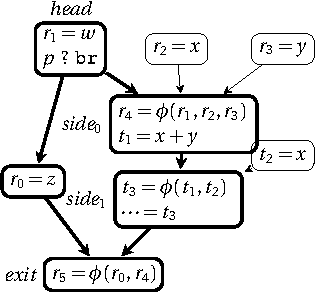
\includegraphics[scale=0.9]{phi_augmentation_a}
  }
  \subfloat[after path-duplication]{
    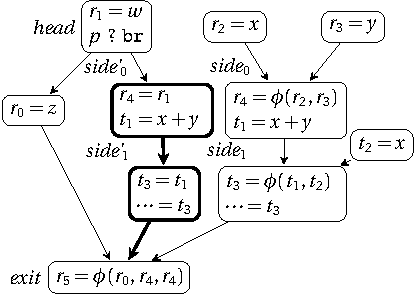
\includegraphics[scale=0.9]{phi_augmentation_b}
  }

  \subfloat[after renaming/copy-folding]{
    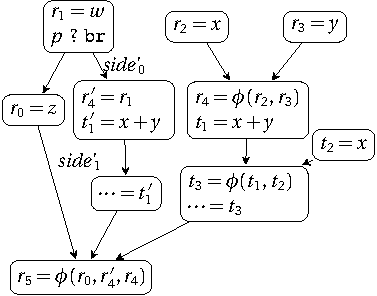
\includegraphics[scale=0.9]{phi_augmentation_c}
  }
  \subfloat[after $\phi$ reduction]{
    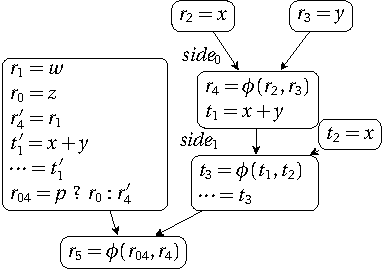
\includegraphics[scale=0.9]{phi_augmentation_d}
  }
  \caption{\label{fig:phi_aug}Path duplication}
\end{figure}


The last transformation, namely the \emph{Conjunctive predicate merge}\index{conjunctive predicate merge}, concerns the if-conversion of a control-flow pattern that sometimes appears on codes to represent logical \texttt{and} or \texttt{or} conditional operations. 
As illustrated in Figure~\ref{fig:phi_merge} the goal is to get rid of side exit edges that avoid a single-entry-node region to be a diamond-DAG. 
As opposed to path duplication, the transformation is actually restricted to a very simple pattern highlighted in Figure~\ref{fig:phi_merge} made up of three distinct basic blocks: \textit{head}, that branches with predicate $p$ to \textit{side}, or \textit{exit}. 
\textit{side}, which is empty, branches itself with predicate $q$ to another basic block outside of the region or \textit{exit}. 
Conceptually, the transformation can be understood as first isolating the outgoing path $p\rightarrow q$ and then if-converting the obtained diamond-DAG.

\begin{figure}[h]
  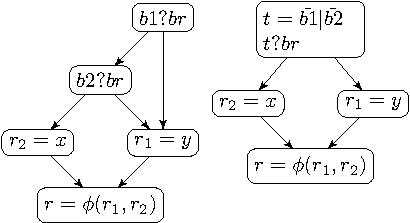
\includegraphics[scale=0.9]{phi_merge}
  \caption{\label{fig:phi_merge}convergent conjunctive merge} 
\end{figure}

Implementing the same framework on a non-SSA form program would require more effort: 
The $\phi$~reduction would do renaming, involving either a global data-flow analysis or the insertion of copies at the \textit{exit} node of the diamond-DAG; 
inferring the minimum amount of {select} operations would also need to maintain liveness information. 
SSA form solves the renaming issue without additional effort and as illustrated in Figure~\ref{fig:pred_min}, the minimality\index{minimal SSA form}\index{pruned SSA form} and the pruned type of the SSA form allows to avoid inserting useless {select} operations.

\begin{figure}[h]
\centering
  \subfloat[if-conversion on minimal SSA] {
   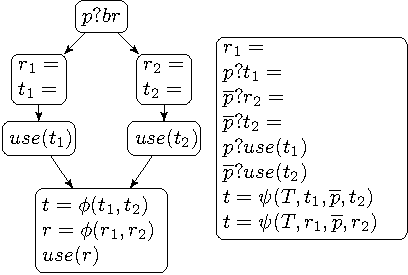
\includegraphics[scale=0.9]{phi_min}
   \label{fig:phi_minimal}}\hfill
  \subfloat[if-conversion on pruned SSA] {
  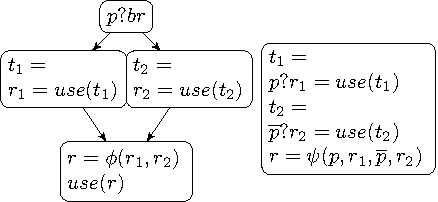
\includegraphics[scale=0.9]{phi_pru}
  \label{fig:phi_pruned}}
\caption{\label{fig:pred_min} SSA predicate minimality}
\label{fig:minimality}
\end{figure}

\subsection{Handling of predicated execution model}

The $\phi$~removal transformation described above considered a speculative execution\index{speculation} model. 
As we will illustrate hereafter, in the context of a predicated execution model, the choice of speculation versus predication\index{predicated execution} is an optimization decision that should not be imposed by the intermediate representation. 
Also, transforming speculated code into predicated code can be viewed as a coalescing\index{coalescing} problem. 
The use of $\psi$-SSA\index{$\psi$-SSA form} (see Chapter~\ref{chapter:psi_ssa}), as the intermediate form of if-conversion, allows to postpone the decision of speculating some code, while the coalescing problem is naturally handled by the $\psi$-SSA destruction phase.

Just as (control) speculating an operation on a control-flow graph means to ignore the control dependence\index{dependence, control-} with the conditional branch, speculating an operation on an if-converted code is the same as removing the data dependence\index{dependence, data-} with the corresponding predicate. 
On the other hand, after register allocation code, speculation adds anti-dependencies\index{dependence, anti-}. 
This trade-off is illustrated in the example of Figure~\ref{fig:pred_versus_spec}: 
For the fully predicated version of the code, the computation of $p$ has to be done before the computations of $x_1$ and $x_2$; 
speculating the computation of $x_1$ removes the dependence with $p$ and allows to execute it in parallel\index{parallel execution} with the test $(a<\hspace{-.6em}?\ b)$; 
if both the computation of $x_1$ and $x_2$ are speculated, they cannot be coalesced and when destruction $\psi$-SSA, the \psifun\index{\psifun} will give rise to some select instruction; 
if only the computation of $x_1$ is speculated, then $x_1$ and $x_2$ can be coalesced to $x$, but then an anti-dependence from $x=a+b$ and $p\cond x = c $ appears that forbids its execution in parallel.

\begin{figure}[h]
\subfloat[predicated code]{
\hspace{0.5cm}\begin{minipage}[b]{2.4cm}\label{subfig:pred_versus_spec:a}
\footnotesize
$ p = (a<\hspace{-.6em}?\ b) $ \\
$ p \cond x_1 = a + b $ \\
$ \overline{p} \cond x_2 = c $ \\
$ x = \psi(p \cond x_1, \overline{p} \cond x_2) $
\end{minipage}
}\hfill
\subfloat[fully speculated]{\index{speculation}
\begin{minipage}[b]{2.4cm}\label{subfig:pred_versus_spec:b1}
\footnotesize
$ p = (a<\hspace{-0.6em}?\ b) $ \\
$ x_1 = a + b $ \\
$ x_2 = c $ \\
$ x = \psi(p \cond x_1, \overline{p} \cond x_2) $ 
\end{minipage}
}\hfill
\subfloat[partially speculated]{
\begin{minipage}[b]{2.7cm}\label{subfig:pred_versus_spec:b2}
\footnotesize
$ p = (a<\hspace{-0.6em}?\ b) $ \\
$ x_1 = a + b $ \\
$ \overline{p} \cond x_2 = c $ \\
$ x = \psi(p\cond x_1, \overline{p} \cond x_2) $ 
\end{minipage}
}\hfill
\subfloat[after coalescing]{
\begin{minipage}[b]{2.3cm}\label{subfig:pred_versus_spec:c}
\footnotesize
$ p = (a<\hspace{-0.6em}?\ b) $ \\
$ x = a + b $ \\
$ \overline{p} \cond x = c $ \\
~
\end{minipage}
}
\caption{\label{fig:pred_versus_spec}Speculation removes the dependency with the predicate but adds anti-dependencies between concurrent computations.}
\end{figure}

In practice, speculation is performed during the $\phi$~removal transformation, whenever it is possible (operations with side effect cannot be speculated) and considered as beneficial. 
As illustrated in Figure~\ref{nested_psi_speculated}, only the operations part of \emph{one} of the diamond-DAG branch are actually speculated. 
This partial speculation leads to manipulating code made up of a mix of predication and speculation.


\begin{figure}
\footnotesize
\subfloat[nested if] {
\begin{minipage}[b]{2cm}
\begin{equation*}
\begin{array}{l}
\iftt (q)\\
\thentt\\
\quad p = (a<\hspace{-0.6em}?\ b)\\~\\
\quad x_1 = a + b\\
\quad \overline{p} \cond x_2 = c\\
\quad x = \psi( x_1, \overline{p} \cond x_2) \\
\quad d_1 = \texttt{f} (x) \\
\elsett\\
\quad d_2 = 3\\
\endtt\\
d = \phi(d_1,d_2)
\end{array}
\end{equation*}\\\vspace{-2.8em}
\end{minipage}
\label{nested_psi}}
\hfill
\subfloat[speculating the \texttt{then} branch] {
\hspace{1cm}
\begin{minipage}[b]{3cm}
~\\\\
$ p = (a<\hspace{-0.6em}?\ b) $ \\~\\
$ x_1 = a + b $ \\
$ \overline{p} \cond x_2 = c $ \\
$ x = \psi(x_1, \overline{p} \cond x_2) $ \\
$ d_1 = \texttt{f} (x) $ \\
~\\
$ \overline{q} \cond d_2 = 3 $ \\
~\\
$ d = \psi(q\cond d_1, \overline{q} \cond d_2) $ 
\end{minipage}
\label{nested_psi_speculated}}
\hfill
\subfloat[predicating both branches] {
\hspace{0.5cm}
\begin{minipage}[b]{3cm}
~\\
$ p = (a<\hspace{-0.6em}?\ b) $ \\
$ s = q\wedge \overline{p} $ \\
$ q \cond x_1 = a + b $ \\
$ s \cond x_2 = c $ \\
$ x = \psi(q \cond x_1, s \cond x_2) $ \\
$ q \cond d_1 = \texttt{f} (x) $ \\~\\
$ \overline{q} \cond d_2 = 3 $ \\~\\
$ d = \psi(q\cond d_1, \overline{q} \cond d_2) $ 
\end{minipage}
\label{nested_psi_predicated}}
\caption{Inner region $\psi$}
\end{figure}

Speculating code is the easiest part as it could be done prior to the actual if-conversion by simply hoisting the code above the conditional branch. 
Still we would like to outline that since \psifuns are part of the intermediate representation, they can be considered for inclusion in a candidate region for if-conversion, and in particular for speculation. 
However, the strength of $\psi$-SSA allows to treat \psifuns just as any other operation. 
Consider the code of Figure~\ref{nested_psi} containing a sub region already processed. 
To speculate the operation $d_1=\texttt{f}(x)$, the operation defining $x$, i.e., the \psifun, also has to be speculated. 
Similarly, all the operations defining the operands $x_1$ and $x_2$ should also be speculated. 
If one of them can produce hazardous execution, then the \psifun cannot be speculated, which forbids in turn the operation $d_1=\texttt{f}(x)$ to be speculated. 
Marking operations that cannot be speculated can be done easily using a forward propagation along def-use chains\index{def-use chains}.

All operations that cannot be speculated, including possibly some \psifuns, should be predicated. 
Suppose we are considering a non-speculated operation we aim at if-converting, that is part of the \texttt{then} branch on predicate $q$. 
Just as for $x_2=c$ in Figure~\ref{nested_psi}, this operation might be already predicated (on $\overline{p}$ here) prior to the if-conversion. 
In that case, a \textit{projection}\index{projection}\index{$\psi$-projection} on $q$ is performed, meaning that instead of predicating $x_2=c$ by $\overline{p}$ it gets predicated by $q\wedge \overline{p}$. 
A \psifun can also be projected on a predicate $q$ as described in Chapter~\ref{chapter:psi_ssa}: 
All gates of each operand are individually projected on $q$. 
As an example, originally non-gated operand $x_1$ gets gated by $q$, while the $\overline{p}$ gated operand $x_2$ gets gated by $s=q\wedge\overline{p}$. 
Note that as opposed to speculating it, predicating a \psifun does not impose to predicate the operation that define its operands. 
The only subtlety related to projection is the generation the new predicate as the logical conjunction of the original guard (e.g., $\overline{p}$)\index{guard} and the current branch predicate (e.g., $q$). 
Here $s$ needs to be computed at some point. 
The heuristic consists in first listing the set of all necessary predicates and then emitting the corresponding code at the earlier place. 
Here, used predicates are $q$, $\overline{q}$, and $q\wedge\overline{p}$. 
$q$ and $\overline{q}$ are already available. 
The earlier place where $q\wedge\overline{p}$ can be computed is just after calculating $p$.

Once operations have been speculated or projected (on $q$ for the \texttt{then} branch, on $\overline{q}$ for the \texttt{else}), each \phifuns at the merge point is replaced by a \psifun: 
operands of speculated operations are placed first and guarded by true; 
operands of projected operations follow, guarded by the predicate of the corresponding branch.

\section{Global analysis and transformations}
\label{sec:if_conversion:hyperblock}
Frequently executed regions are rarely just composed of simple \texttt{if-then-else-end} control-flow regions but processors have limited resources: 
the number of registers will determine the acceptable level of data dependencies to minimize register pressure; 
the number of predicate registers will determine the depth of the if-conversion so that the number of conditions does not exceed the number of available predicates; 
the number of processing units will determine the number of instructions that can be executed simultaneously. 
The inner-outer incremental process advocated in this chapter allows to evaluate precisely the profitability of if-conversion.

\subsection{SSA incremental if-conversion algorithm}

%% For each basic block considered within the region, a predicate must be computed and assigned to the corresponding instructions. Those predicate computations introduce new instructions and new data dependencies, that need to be controlled while the region is been if-converted.

The algorithm takes as input a CFG in SSA form and applies incremental reductions using the list of candidate conditional basic blocks sorted in post-order. 
Each basic block in the list designates the head of a sub-graph that can be if-converted using the transformations described in Section~\ref{sec:basic}. 
Post-order traversal allows to process each region from the inner to the outer. 
When the if-converted region cannot grow anymore because of resources, or because a basic block cannot be if-converted, then the next sub-graph candidate is considered until all the CFG is explored.
%
%% During this incremental process, since nested regions are already predicated when evaluating the if-conversion of a branch, all the side effects, such as new predicate merging instructions, new conditional moves merging flow or new data dependencies, will be accounted to evaluate the profitability.
%
Note that as the reduction proceeds, maintaining SSA\index{incremental update, of SSA} can be done using the general technique described in Chapter~\ref{chapter:repair_maintain_ssa_after_optimization}. 
Basic local ad hoc updates can also be implemented instead.

Consider for example the CFG from reported in Figure~\ref{fig:wc1}. 
The exit node $\textit{BB}7$, and basic block $\textit{BB}3$ that contains a function call cannot be if-converted (represented in gray). 
The post-order list of conditional blocks (represented in bold) is [$\textit{BB}11$, $\textit{BB}17$, $\textit{BB}16$, $\textit{BB}14$, $\textit{BB}10$, $\textit{BB}9$, $\textit{BB}6$, $\textit{BB}2$]. 
(1)~The first candidate region is composed of $\{\textit{BB11}, \textit{BB}2, \textit{BB}12\}$; 
$\phi$-reduction can be applied, promoting the instructions of $\textit{BB}12$ in $\textit{BB}11$; 
$\textit{BB}2$ becomes the single successor of $\textit{BB}11$. 
(2)~The region headed by $\textit{BB}17$ is then considered; 
$\textit{BB}19$ cannot yet be promoted because of the side entries coming both from $\textit{BB}15$ and $\textit{BB}16$; 
$\textit{BB}19$ is duplicated into a $\textit{BB}19'$ with $\textit{BB}2$ as successor; 
$\textit{BB}19'$ can then be promoted into $\textit{BB}17$. 
(3)~The region headed by $\textit{BB}16$ that have now $\textit{BB}17$ and $\textit{BB}19$ as successors is considered; 
$\textit{BB}19$ is duplicated into $\textit{BB}19''$, so as to promote $\textit{BB}17$ and $\textit{BB}19'$ into $\textit{BB}16$ through $\phi$-reduction; 
$\textit{BB}19'$ already contains predicated operations from the previous transformation, so a new merging predicate is computed and inserted.
After the completion of $\phi$-removal, $\textit{BB}16$ has a unique successor, $\textit{BB}2$. 
(4)~$\textit{BB}14$ is the head of the new candidate region;
Here, $\textit{BB}15$ and $\textit{BB}16$ can be promoted.
Again since $\textit{BB}16$ contains predicated and predicate setting operations, a fresh predicate must be created to hold the merged conditions. 
(5)~$\textit{BB}10$ is then considered; 
$\textit{BB}14$ needs to be duplicated to $\textit{BB}14'$. 
The process finishes with the region head $\textit{BB}9$.

\begin{figure}
  \subfloat[Initial] {
    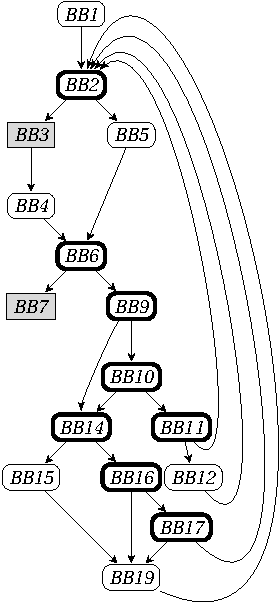
\includegraphics[scale=0.7]{graph_a}
    \label{fig:wc1}}
  \subfloat[If-conversion] {
    \hspace{1em}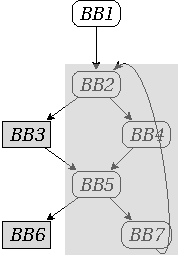
\includegraphics[scale=0.7]{graph_b}\hspace{1em}
    \label{fig:wc2}}
  \subfloat[Tail duplication] {
    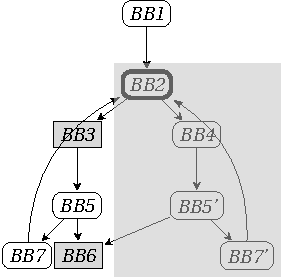
\includegraphics[scale=0.7]{graph_c}
    \label{fig:wc3}}
\caption{\label{fig:wc example}If-conversion of \texttt{wc} (word count program). Basic blocks in the gray region cannot be if-converted. Tail duplication can be used to exclude \textit{BB3} from the to-be-if-converted region.}
\end{figure}


\subsection{Tail duplication}

Just as shown in Figure~\ref{fig:wc example}, some basic blocks (such as \textit{BB3}) may have to be excluded from the region to if-convert. 
\emph{Tail duplication}\index{tail duplication}  can be used for this purpose. 
Similar to path duplication\index{path duplication} described in Section~\ref{sec:basic}, the goal of tail duplication is to get rid of incoming edges of a region to if-convert. 
This is usually done in the context of hyperblock formation\index{hyperblock formation}, such technique consists in, as opposed to the inner-outer incremental technique described in this chapter, to if-convert a region in ``one shot''. 
Consider again the example of Figure~\ref{fig:wc1}, and suppose the set of selected basic blocks defining the region to if-convert consists of all basic blocks from \textit{BB2} to \textit{BB19} excluding \textit{BB3}, \textit{BB4}, and \textit{BB7}. 
Getting rid of the incoming edge from \textit{BB4} to \textit{BB6} is possible by duplicating all basic blocks of the region reachable from \textit{BB6} as shown in Figure~\ref{fig:wc2}.

Consider a region $\cal R$ made up of a set of basic blocks, a distinguished one $\textit{entry}$ and the others denoted $\left(B_i\right)_{2\leq i\leq n}$, such that any $B_i$ is reachable from \textit{entry} in $\cal R$. 
Suppose a basic block $B_s$ has some predecessors $\textit{out}_1,\ \dots,\ \textit{out}_m$ that are not in $\cal R$. 
Tail duplication consists in: 
(1)~for all $B_j$ (including $B_s$) reachable from $B_s$ in $\cal R$, create a basic block $B'_j$ as a copy of $B_j$; 
(2)~any branch from $B'_j$ that points to a basic block $B_k$ of the region is rerouted to its duplicate $B'_k$; 
(3)~any branch from a basic block $\textit{out}_k$ to $B_s$ is rerouted to $B'_s$. 
In our example, we would have $\textit{entry}=\textit{BB2}$, $B_s=\textit{BB6}$, and $\textit{out}=\textit{BB4}$.

A global approach would just do as in Figure~\ref{fig:wc3}: 
First select the region; 
Second, get rid of the incoming edges using tail duplication.
Finally perform if-conversion of the whole region in one shot. 
We would like to point out that there is no phasing issue with tail duplication. 
To illustrate this point, consider the example of Figure~\ref{fig:hyper1} where \textit{BB2} cannot be if-converted. 
The selected region is made up of all other basic blocks. 
Using a global approach as in standard hyperblock formation, tail duplication would be performed prior to any if-conversion. 
This would lead to the CFG of Figure~\ref{fig:hyper2}. 
Note that a new node, \textit{BB}7, has been added here after the tail duplication by a process called branch coalescing\index{branch coalescing}. 
Applying if-conversion on the two disjoint regions respectively head by \textit{BB4} and \textit{BB4'} would lead to the final code shown if Figure~\ref{fig:hyper3}. 
Our incremental scheme would first perform if-conversion of the region head by \textit{BB4}, leading to the code depicted in Figure~\ref{fig:hyper4}. 
Applying tail duplication to get rid of the side entry from \textit{BB2} would lead to exactly the same final code as shown in Figure~\ref{fig:hyper5}.

\begin{figure}[h]
  \subfloat[initial] {
    \hspace{2em}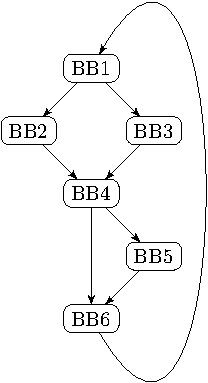
\includegraphics[scale=0.7]{hyper1}\hspace{2em}
    \label{fig:hyper1}}\hfill
  \subfloat[tail duplication] {
    \hspace{2em}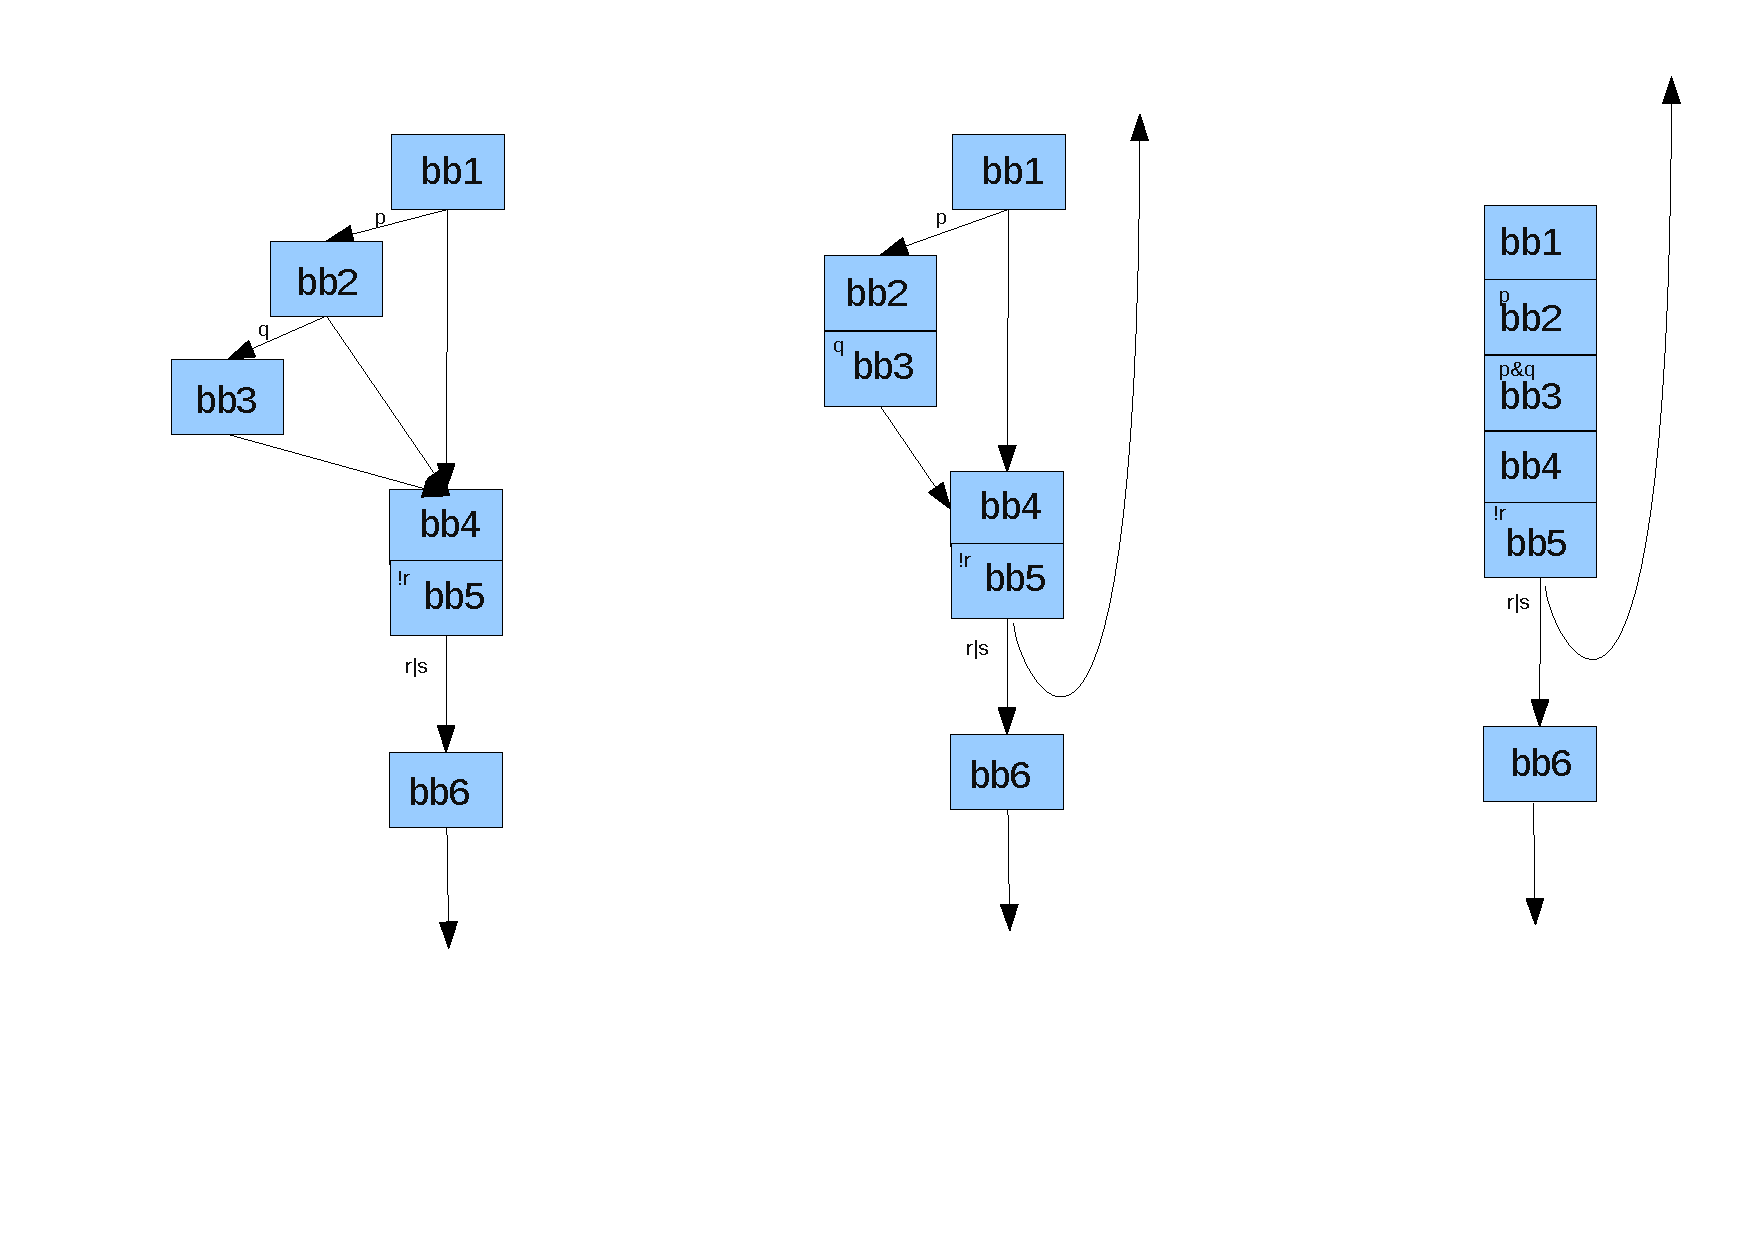
\includegraphics[scale=0.7]{hyper2}\hspace{2em}
    \label{fig:hyper2}}\hfill
  \subfloat[if-convertion] {
    \hspace{2em}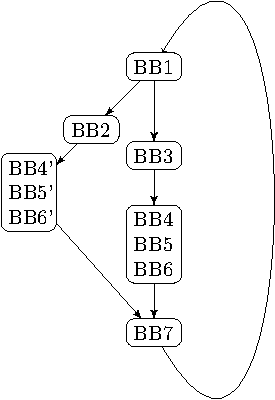
\includegraphics[scale=0.7]{hyper3}\hspace{2em}
    \label{fig:hyper3}}\\
  \subfloat[initial] {
    \hspace{2em}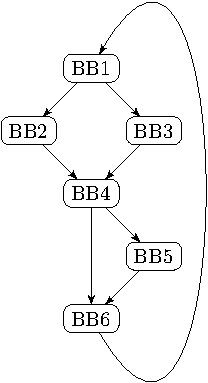
\includegraphics[scale=0.7]{hyper1}\hspace{2em}
    }\hfill
  \subfloat[if-conversion] {
    \hspace{2em}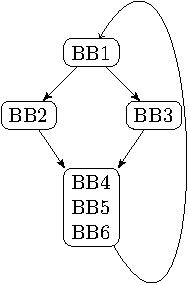
\includegraphics[scale=0.7]{hyper4}\hspace{2em}
    \label{fig:hyper4}}\hfill
  \subfloat[tail duplication] {
    \hspace{2em}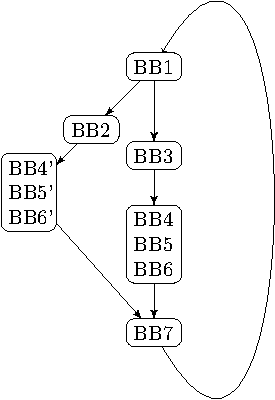
\includegraphics[scale=0.7]{hyper3}\hspace{2em}
    \label{fig:hyper5}}
 \caption{Absence of phasing issue for tail duplication\label{fig:hyper}}
\end{figure}


\subsection{Profitability}

Fusing execution paths can over commit the architectural ability to execute in parallel the multiple instructions: 
Data dependencies and register renaming introduce new register constraints. 
Moving operations earlier in the instruction stream increases live-ranges. 
Aggressive if-conversion can easily exceed the processor resources, leading to excessive register pressure or moving infrequently used long latency instructions into the critical path. 
The prevalent idea is that a region can be if-converted if the cost of the resulting if-converted basic block is smaller than the cost of each basic block of the region taken separately weighted by its execution probability. 
To evaluate those costs, we consider all possible paths impacted by the if-conversion.

For all transformations but the conjunctive predicate merge, there are two such paths starting at basic block \textit{head}. 
For the code of Figure~\ref{fig:paths_reduction}, we would have $\textit{path}_p=[\textit{head}, B_1, \textit{exit}[$ and $\textit{path}_{\overline{p}}=[\textit{head}, B'_1, B'_2, \textit{exit}[$ of respective probability $\proba{p}$ and $\proba{\overline{p}}$. 
For a path $\textit{P}_q=[B_0, B_1, \dots, B_n[$ of probability $\proba{q}$, its cost is given by $\cost{\textit{P}_q}=\proba{q}\times \sum_{i=0}^{n-1} \cost{[B_i,B_{i+1}[}$ where $\cost{[B_i,B_{i+1}[}$ represents the cost of basic block $\cost{[B_i]}$ estimated using its schedule height plus the branch latency $\brlat$, if the edge $(B_i,B_{i+1})$ corresponds to a conditional branch, 0 otherwise. 
Note that if $B_i$ branches to $S_q$ on predicate $q$, and falls through to $S_{\overline{q}}$, $\cost{B_i}=\proba{q}\times \left(\cost{[B_i,S_q[}\right)+\proba{\overline{q}}\times \left(\cost{[B_i,S_{\overline{q}}[}\right)=\cost{[B_i]}+\proba{q}\times\brlat$.

Let $\textit{path}_p=[\textit{head}, B_1, \dots, B_n, \textit{exit}[$ and $\textit{path}_{\overline{p}}=[\textit{head}, B'_1, \dots, B'_m, \textit{exit}[$ be the two paths with the condition taken branch on $p$. 
Then, the overall cost before if-conversion simplifies to
$$\textsf{cost}_{\textsf{control}}=\cost{\textit{path}_p}+\cost{\textit{path}_{\overline{p}}}=\cost{[\textit{head}]} + \proba{p}\times\left(\brlat+\sum_{i=0}^n \cost{[B_i]}\right) + \proba{\overline{p}}\times\sum_{i=0}^m \cost{[B'_i]}$$
This is to be compared to the cost after if-conversion
$$\textsf{cost}_{\textsf{predicated}}=\cost{\left[\textit{head} \circ \left(\bigcirc_{i=1}^n B_i\right)\circ \left(\bigcirc_{i=1}^m B'_i\right)  \right]}$$
where $\circ$ is the composition function that merges basic blocks together, removes associated branches and creates the predicate operations. 

\begin{figure}[h]
  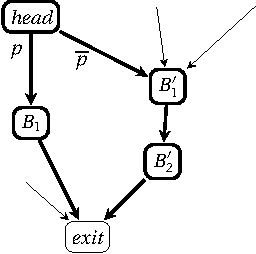
\includegraphics[scale=0.7]{paths_reduction_a.pdf}\hspace{0.5cm}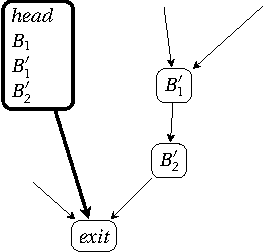
\includegraphics[scale=0.7]{paths_reduction_b.pdf}
  \caption{$\phi$ reduction\label{fig:paths_reduction}}
\end{figure}

The profitability for the logical conjunctive merge of Figure~\ref{fig:paths_convergent} can be evaluated similarly. 
There are three paths impacted by the transformation: 
$\textit{path}_{p\wedge q}=[\textit{head}, \textit{side}, B_1[$, $\textit{path}_{p\wedge \overline{q}}=[\textit{head}, \textit{side}, \textit{exit}[$, and $\textit{path}_{\overline{p}}=[\textit{head}, \textit{exit}[$ of respective probability $\proba{p\wedge q}$, $\proba{p\wedge \overline{q}}$, and $\proba{\overline{p}}$. 
The overall cost before the transformation (if branches are on $p$ and $q$) $\cost{\textit{path}_{p\wedge q}}+\cost{\textit{path}_{p\wedge \overline{q}}}+\cost{\textit{path}_{\overline{p}}}$ simplifies to
$$\textsf{cost}_{\textsf{control}}=\cost{\textit{head}}+\cost{\textit{side}}=\cost{\textit{[head]}}+\proba{p}\times (1+\proba{q})\times\brlat$$
which should be compared to (if the branch on the new \textit{head} block is on $p \wedge q$)
$$\textsf{cost}_{\textsf{predicated}}=\cost{\textit{head}\circ \textit{side}}=\cost{[\textit{head}\circ \textit{side}]}+\proba{p}\times\proba{q}\times \brlat$$
\begin{figure}[h]
  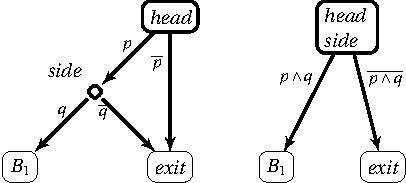
\includegraphics[scale=0.7]{paths_convergent.pdf}
  \caption{conjunctive predicate merge\label{fig:paths_convergent}}
\end{figure}

Note that if $\proba{p}\ll 1$, emitting a conjunctive merge might not be beneficial. 
In that case, another strategy such as path duplication from the \textit{exit} block will be evaluated. 
Profitability for any conjunctive predicate merge (disjunctive or conjunctive; 
convergent or not) is evaluated similarly.

A speed oriented objective function needs the target machine description to derive the instruction latencies, resource usage and scheduling constraints. 
The local dependencies computed between instructions are used to compute the dependence height. 
The branch probability is obtained either from static branch prediction heuristics, profile information or user inserted directives. 
Naturally, this heuristic can be either pessimistic, because it does not take into account new optimization opportunities introduced by the branch removal or explicit new dependencies, or optimistic because of bad register pressure estimation leading to register spilling on the critical path, or uncertainty in the branch prediction. 
But since the SSA incremental if-conversion framework reduces the scope for the decision function to a localized part of the CFG, the size and complexity of the inner region under consideration makes the profitability a comprehensive process. 
This cost function is fast enough to be reapplied to each region during the incremental processing, with the advantage that all the instructions introduced by the if-conversion process in the inner regions, such as new predicate merging instructions or new temporary pseudo-registers, can be taken into account.

\section{Concluding remarks and further reading} 
We presented in this chapter how an if-conversion algorithm can take advantage of the SSA properties to efficiently assign predicates and lay out the new control flow in an incremental, inner-outer process. 
As opposed to the alternative top-down approach, the region selection can be reevaluated at each nested transformation, using local analysis. 
Hyperblocks~\cite{Mahlke:1992:ECS:144965.144998} was proposed as the primary if-converted scheduling framework, excluding basic blocks which do not justify their inclusion into the if-converted flow of control.
Region selection and if-conversion can be performed as a single pass, hyperblocks being created lazily, using well-known techniques such as tail duplication or branch coalescing only when the benefit is established. 
Predication and speculation are often presented as two different alternatives for if-conversion. They can coexist in an efficient if-conversion process such that every model of conditional execution is accepted in the same framework, thanks to the conditional moves and $\psi$ \cite{Stoutchinin:2001:MICRO} transformations.















